
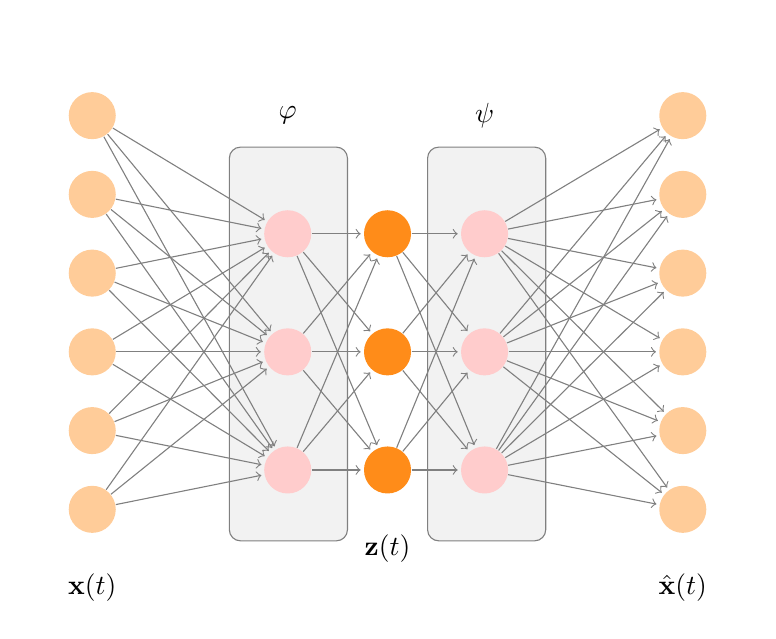
\begin{tikzpicture}[shorten >=1pt,->,draw=black!50, node distance=2cm]
\tikzstyle{every pin edge}=[<-,shorten <=1pt]
\tikzstyle{neuron}=[circle,fill=purple!50,minimum size=17pt,inner sep=0pt]
\tikzstyle{input neuron}=[neuron, fill=orange!40];
\tikzstyle{output neuron}=[neuron, fill=orange!40];
\tikzstyle{hidden neuron}=[neuron, fill=red!20];
\tikzstyle{annot} = [text width=4em, text centered]

% Define layer separation
\def\layersep{2.5cm}

% Draw the input layer nodes
\foreach \name / \y in {1,...,6}
  \node[input neuron] (I-\name) at (0,-\y) {};

% Draw the hidden layer box for phi
\node[draw, rectangle, minimum width=1.5cm, minimum height=5cm, fill=gray!10, rounded corners] (phi) at (\layersep-0.25,-3.9) {};

% Draw the hidden layer nodes inside the box for phi
\foreach \name / \y in {1,...,3}
  \node[hidden neuron] (H-\name) at (\layersep-0.5,-1.5*\y-1) {};

% Draw the hidden layer box for psi
\node[draw, rectangle, minimum width=1.5cm, minimum height=5cm, fill=gray!10, rounded corners] (psi) at (2*\layersep+0.25,-3.9) {};

% Draw the hidden layer nodes inside the box for psi
\foreach \name / \y in {1,...,3}
  \node[hidden neuron] (H2-\name) at (2*\layersep-0.5,-1.5*\y-1) {};

% Draw the latent layer nodes
\foreach \name / \y in {1,...,3}
  \node[hidden neuron, fill=orange!90] (Z-\name) at (1.5*\layersep,-1.5*\y-1) {};

% Draw the output layer nodes
\foreach \name / \y in {1,...,6}
  \node[output neuron] (O-\name) at (3*\layersep,-\y) {};

% Connect every node in the input layer with every node in the hidden layer.
\foreach \source in {1,...,6}
  \foreach \dest in {1,...,3}
    \path (I-\source) edge (H-\dest);

% Connect every node in the hidden layer with every node in the latent layer.
\foreach \source in {1,...,3}
  \foreach \dest in {1,...,3}
    \path (H-\source) edge (Z-\dest);

% Connect every node in the latent layer with every node in the hidden layer.
\foreach \source in {1,...,3}
  \foreach \dest in {1,...,3}
    \path (Z-\source) edge (H2-\dest);

% Connect every node in the hidden layer with every node in the output layer.
\foreach \source in {1,...,3}
  \foreach \dest in {1,...,6}
    \path (H2-\source) edge (O-\dest);

% Annotate the layers
\node[annot,above of=H-1, node distance=1.5cm] (phi_text) {$\varphi$};
\node[annot,above of=H2-1, node distance=1.5cm] (psi_text) {$\psi$};
\node[annot,above of=I-1, node distance=1cm] (input) {};
\node[annot,above of=O-1, node distance=1cm] (output) {};

% Annotate the layers with x(t), z(t), and \hat{x}(t)
\node[annot,below of=I-6, node distance=1cm] (input) {$\mathbf{x}(t)$};
\node[annot,below of=Z-3, node distance=1cm] (latent) {$\mathbf{z}(t)$};
\node[annot,below of=O-6, node distance=1cm] (output) {$\hat{\mathbf{x}}(t)$};

\end{tikzpicture}
